\documentclass[12pt,a4paper]{article}

\usepackage{graphicx}
\usepackage{amsmath}
\usepackage{amsfonts}
\usepackage[backend=biber, style=numeric, sorting=none]{biblatex}
\usepackage[linesnumbered,ruled,vlined]{algorithm2e}
\usepackage{hyperref}
\addbibresource{bibliography.bib} % Specify the .bib file


\setlength{\topmargin}{0.0in}
\setlength{\oddsidemargin}{0.33in}
\setlength{\textheight}{9.0in}
\setlength{\textwidth}{6.0in}
\renewcommand{\baselinestretch}{1.25}


\title{Modelling the UK's Renewable Energy Infrastructure as a Capacitated Facility Location Problem using a Lagrangian Relaxation Heuristic}
\author{Integer Programming}
\date{Candidate Number: 1090497}

\begin{document}

\maketitle

\thispagestyle{empty}

\newpage
\setcounter{page}{1}


\section{Introduction}
The Facility Location Problem (FLP) is a mathematical optimisation problem that aims 
to find the locations  a set of supply facilities can serve a set of demand sites at the lowest cost. 
Typically two types of cost are associated with the problem: 
\textit{setup costs} which are required to setup a facility and 
\textit{supply/connection costs} associated
with a facility meeting the demand of a given demand centre. Specific instances of the FLP 
are the Uncapacitated Facility Location Problem (UFLP) in which facilities have an unlimited supply of product, and 
the Capacitated Facility Location Problem (CFLP) in which facilities have a capacity on how much 
they can supply \cite{wu2006capacitated}. \par

Lots of challenges encountered in logistics and operations research lend themselves to 
formulation as CFLP problems. Canonical examples include determing locations for factories or warehouses 
to be established. Another set of problems that lend themselves to this formulation are those encountered in 
Energy Systems Modelling (ESM), a field employing the use of computational models to support policy
decisions regarding energy infrastructure. Such models typically aim at obtaining cost/benefit estimates
regarding changes to existing energy infrastructure or policy; for example, the consequences of subsidies, impact of new supply lanes 
and effects of introducing new energy generation and storage technologies. As many governments have
launched projects aiming to transition away from fossil fuels and replace these with renewables, 
energy systems modelling is now also employed in cost estimation, technology selection and pathway
estimation \cite{hoffmann2024review} \cite{nakata2011application}.\par

In this report we present a modification of the CFLP that is applied to determine optimal site choice 
for renewable energy infrastructure, which in this report we call the Energy Systems Location Problem (ESLP).
We then derive a Lagrangian Relaxation Heuristic (LR Heuristic) that is used to approximate solutions to this problem,
partially inspired by \cite{wu2006capacitated}, and apply it to a specific case: selecting optimal technologies and sites for UK 
renewable energy technologies that can meet the UK's energy demands. This report will be organised as follows. 
In Section \ref{sec:2} we first outline the CFLP, and then present a modified version to fit requirements for energy systems modelling 
and obtain the ESLP. We then derive the LR heuristic that will be tested. In Section \ref{sec:3} we describe the
case study we will test the ESLP and LR Heuristic on and how the data was obtained and processed.
We then present results, comparing a direct implementation of the ESLP to the derived LR Heuristic.



\section{The CFLP, ESLP and LR heuristic}\label{sec:2}
\subsection{CFLP Definition}
The CFLP involves determining the optimal locations to establish supply sites that meet demand at multiple
sites, while minimising the total costs incurred. Costs are facility setup costs and supply costs,
and each supply site is subject to capacity constraints, meaning there is an upper bound on how much 
supply a site can provide.

Mathematically the problem is formulated in the following way. First, let $S$ be the set of supply sites, 
indexed by $s \in S$ and let $D$ be the set of demand sites, indexed by $d \in D$. By $c_{s,d}$ we denote the
cost associated with site s supplying site d and by $f_s$ we denote the setup cost associated with constructing site $s$.
By $u_s$ we denote the maximum capacity that site $s$ can supply overall and by $r_d$ we denote the amount of demand 
required to be met at at site $d$. The decision variables in this problem are $x_{s,d} \in \mathbb{R}_{\geq 0}$, denoting the amount 
supplied by supply site $s$ to demand site $d$, and $y_s \in \mathbb{B}$, a binary variables indicating whether site 
$s$ has been constructed. With these defined the problem can be formulated as such:

\begin{subequations}\label{eq:CFLP}
    \begin{align}
    \text{CFLP: } \quad \quad \min \quad & \sum_{s \in S} f_s y_s + \sum_{s \in S}\sum_{d \in D} c_{s,d} x_{s,d} \label{eq:CFLP_obj}\\
    \text{subject to: } \sum_{s \in S} x_{s,d} &\geq r_d, \quad \forall d \in D,\label{eq:CFLP_dem}\\
    \sum_{d \in D} x_{s,d} &\leq u_s y_s, \quad \forall s \in S,\label{eq:CFLP_cap}\\
    y_s &\in \{0, 1\}, \quad \forall s \in S,\label{eq:CFLP_y}\\
    x_{s,d} &\geq 0, \quad \forall s \in S, \forall d \in D.\label{eq:CFLP_x}
    \end{align}
\end{subequations}


Equation \ref{eq:CFLP_dem} imposes the demand constraint, i.e. that the amount supplied by all supply sites $s$ 
to a site $d$ must be greater than or equal to the demand at site $d$ for all $d \in D$. Equation \ref{eq:CFLP_cap} 
imposes both the build constraint and the capacity constraint, i.e. that a supply site $s$ cannot provide any supply
if it has not been constructed (recall $y_s$ is binary), and that a supply site $s$ 
cannot provide a supply in excess of its total capacity $u_s$. Equations \ref{eq:CFLP_x} and 
\ref{eq:CFLP_y} are the integrality constraints. 

We now discuss the problem of energy systems modelling and adapt the general CFLP formulation to 
consider this case.

\subsection{Energy Systems Modelling - formulating the ESLP}

The challenge of determining optimal build sites,technology mixes or supply routes 
for energy systems has seen a number of mixed-integer linear formulations proposed
\cite{hoffmann2024review}. To introduce and motivate modelling energy site locations
and technology choices using a CFLP framework we illustrate using a simplistic example. \par

\begin{figure}[H]
    \centering
    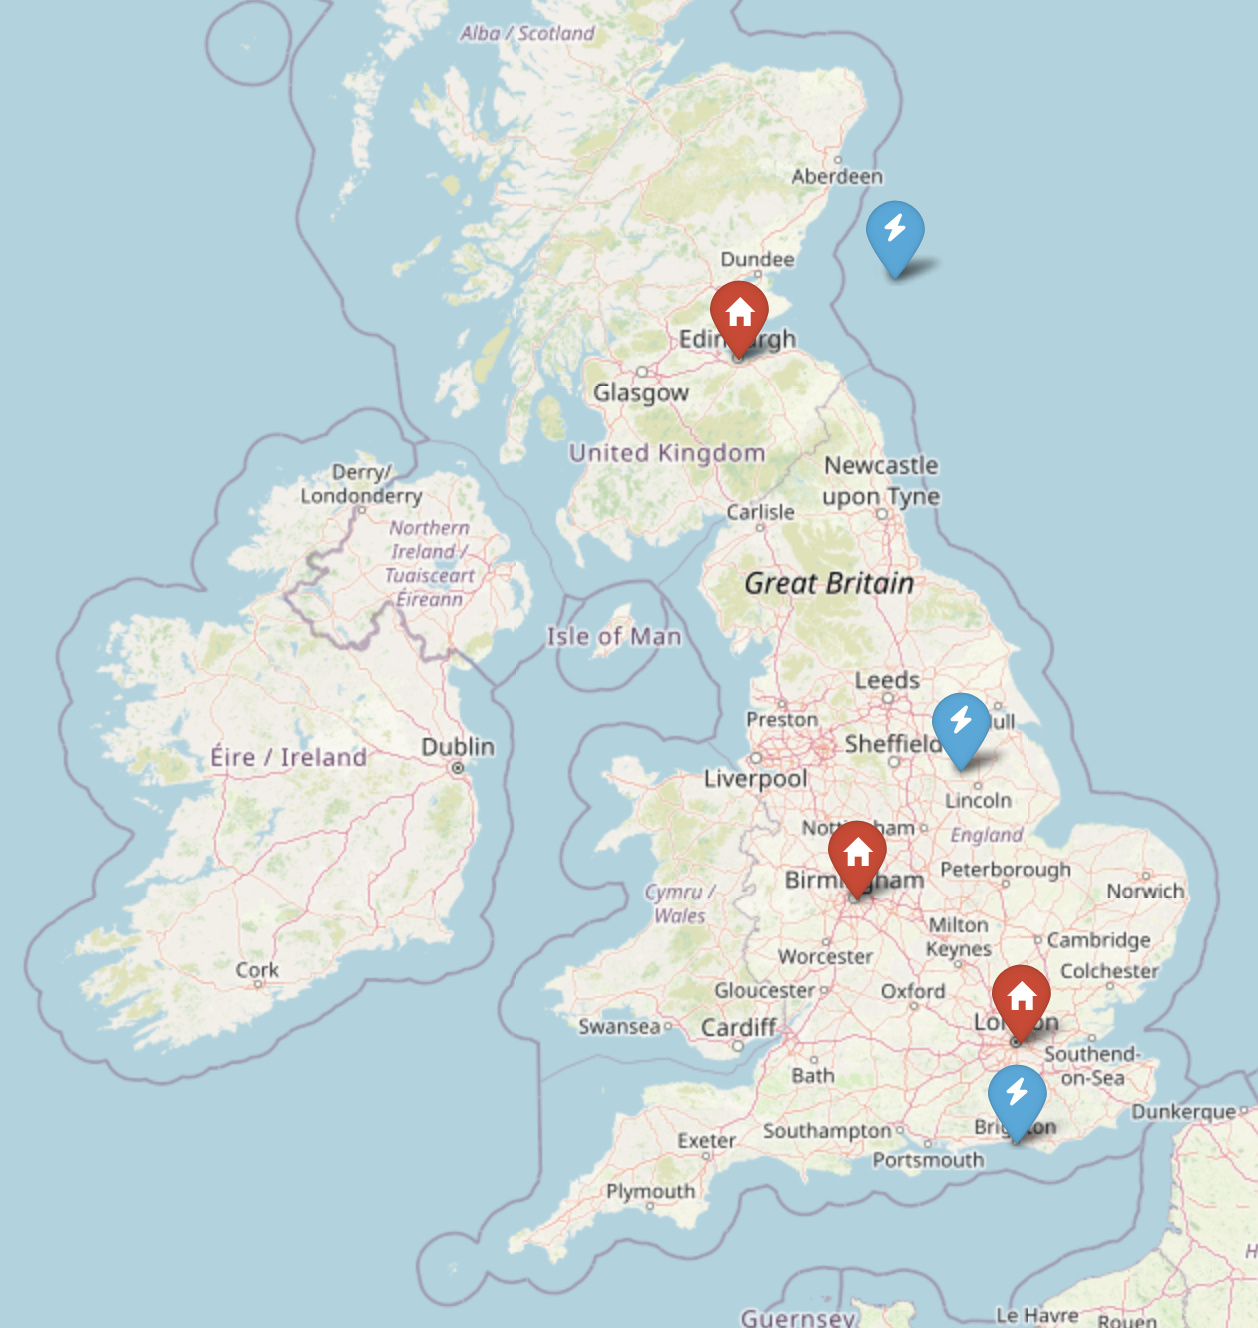
\includegraphics[width=0.4\textwidth]{figures/intro_example.png}
    \caption{Basic Energy Systems Problem}
    \label{fig:intro_plot}
\end{figure}


Figure \ref{fig:intro_plot} plots 3 potential renewable energy power plant sites marked with blue power
icons and 3 demand sites requiring power with red house markers. Each demand site has an associated energy
demand typically measured in MWh or GWh depending on the scope being considered, and each power plant
has an associated cost in supplying energy that can be measured in financial cost per GWh. Each supply site
also has its own associated maximum capacity it can supply. We derive estimates for these associated 
costs and capacities in Section \ref{sec:data_and_processing} when outlining the case study, but 
at this point it is sufficient to see
that if we wish to identify which set of renewable energy sites best meeets energy demands at the
lowest cost, then framing this as a CFLP is a natural choice. \par

However, energy systems need to optimise for varying demand over some time horizon.
Energy demands fluctuate, and depending on the application, time windows can be considered over hourly,
seasonal or annual time periods. Any analysis aiming to optimise this system should consider minimising 
cost to meet fluctuating demand, and this the CFLP does not consider. Similarly, supply costs can also vary
over time.
Therefore, we propose a modification to the CFLP that considers fluctuating demand, which in this report
is called the Energy Systems Location Problem (ESLP). Further modifications could have been considered, 
and these are discussed in Section \ref{sec:future_modifications}.\par

To setup the ESLP, we again consider supply and demand sets $S$ and $D$, again indexed by $s \in S$ and $d \in D$. 
We also add the set $T$ indexed by $t \in T$ to the problem, which represents the set of time points along which 
this problem is being considered. By $c_{s, d, t}$ we describe the cost incurred for supply site $s$ to supply demand 
site $d$ with a unit of demand at time $t$. As in the CFLP, $f_s$ denotes the cost associated with setting up site $s$.
Setup is assumed to have taken place initially (although cases where setup can occur at different times
could be a valuable modification for capital planning, see Section \ref{sec:future_modifications}).
$u_{s}$ denotes the maximum capacity of site $s$ through a single time period $t$ and $r_{d, t}$ denotes the demand required to be met at site 
d at time t. Our decision variables now are $x_{s, d, t} \in \mathbb{R}_{\geq 0}$ which describes the amount supplied by 
supply site $s$ to demand site $d$ at time $t$, and $y_s \in \mathbb{B}$ which indicates whether supply site $y$ is 
constructed or not. The ESLP problem is therefore:

\begin{subequations}\label{eq:ESLP}
    \begin{align}
    \text{ESLP: } \quad \quad \min \quad & \sum_{s \in S} f_s y_s + \sum_{s \in S}\sum_{d \in D}\sum_{t \in T} c_{s,d,t} x_{s,d, t} \label{eq:ESLP_obj}\\
    \text{subject to: } & \sum_{s \in S} x_{s,d,t} \geq r_{d,t} \quad \forall d \in D, \forall t \in T, \label{eq:ESLP_dem}\\
    & \sum_{d \in D} x_{s,d, t} \leq u_{s} y_s, \quad \forall s \in S, \forall t \in T, \label{eq:ESLP_cap}\\
    & y_s \in \{0, 1\}, \quad \forall s \in S,\label{eq:ESLP_y}\\
    & x_{s,d,t} \geq 0, \quad \forall s \in S, \forall d \in D, \forall t \in T.\label{eq:ESLP_x}
    \end{align}
\end{subequations}

\ref{eq:ESLP_obj} is the objective function to be minimised for the ESLP. \ref{eq:ESLP_dem} encodes the requirements that
at all points in time the demand at demand site d must be met. \ref{eq:ESLP_cap} says that at no points in time can a 
supply site exceed its capacity. \ref{eq:ESLP_x} and \ref{eq:ESLP_y} represent the integrality constraints.


\subsection{Lagrangian Relaxation}
Lagrangian relaxation (LR) has been used extensively in CFLP problems ADD THE CITATIONS HERE. It is 
fundamentally a technique for obtaining a lower bound on the original problem, and solving the LR
of a problem commonly forms a step in algorithms aiming to find approximate solutions.
The LR reformulates a problem by moving one of the constraints into the objective function and 
weights the new term with a set of $\lambda \geq 0$ parameters. The LR of a problem can therefore violate the
constraint but is penalised for doing so. 
Crucially, the solution of the LR provides a lower bound on the optimal value of the original solution. 
In this report we consider moving the capacity constraint \ref{eq:ESLP_cap} in the ESLP \ref{eq:ESLP} into 
the objective function, obtaining the LR ESLP.

\begin{subequations}\label{eq:LR_ESLP}
    \begin{align}
    \text{LR ESLP: } \min \quad \sum_{s \in S} f_s y_s + &\sum_{s \in S}\sum_{d \in D}\sum_{t \in T} c_{s,d,t} x_{s,d,t} + \sum_{s \in S}\sum_{t \in T} \lambda_{s,t} \left( \sum_{d \in D} x_{s,d,t} - u_s y_s \right) \label{eq:LR_ESLP_obj} \\
    \text{subject to: } &\sum_{s \in S} x_{s,d,t} \geq r_{d,t}, \quad \forall d \in D, \forall t \in T, \label{eq:LR_ESLP_dem} \\
    &y_s \in \{0, 1\}, \quad \forall s \in S, \label{eq:LR_ESLP_y} \\
    &x_{s,d,t} \geq 0, \quad \forall s \in S, \forall d \in D, \forall t \in T. \label{eq:LR_ESLP_x}
    \end{align}
\end{subequations}


Here we have introduced the parameters $\lambda_{s, t} \geq 0 \quad \forall S, \forall T$ that play the role of penalising any supply sites $s$ which exceed their capacity constraints at time $t$.
A proof that any minimised objective function value of \ref{eq:LR_ESLP_obj} for given values of $\lambda_{s,t}$ is a lower bound on the objective function of the ESLP \ref{eq:ESLP_obj} is as follows.\par


Let

\begin{equation}\label{eq:Lagrangian}
    \begin{aligned}
        \mathcal{L}(x,y,\lambda) &= \sum_{s \in S} f_s y_s + \sum_{s \in S}\sum_{d \in D}\sum_{t \in T} c_{s,d,t} x_{s,d,t} + \sum_{s \in S}\sum_{t \in T} \lambda_{s,t} \left( \sum_{d \in D} x_{s,d,t} - u_s y_s \right) \\
        &= Z(x, y) + \sum_{s \in S}\sum_{t \in T} \lambda_{s,t} \left( \sum_{d \in D} x_{s,d,t} - u_s y_s \right)
    \end{aligned}    
\end{equation}

where $Z(x,y)$ is the objective function \eqref{eq:ESLP_obj} in the original ESLP.

From the capacity constraints in the ESLP \eqref{eq:ESLP_cap}, we obtain that:

\begin{equation}\label{eq:capacity_constraints}
    \sum_{d \in D} x_{s,d,t} \leq u_{s,t} y_s, \quad \forall s \in S, \forall t \in T,
\end{equation}

which can be rewritten as:

\begin{equation}\label{eq:capacity_constraints_rearranged}
    \sum_{d \in D} x_{s,d,t} - u_{s,t} y_s \leq 0, \quad \forall s \in S, \forall t \in T.
\end{equation}

Multiplying both sides of \eqref{eq:capacity_constraints_rearranged} by the non-negative Lagrange multipliers $\lambda_{s,t} \geq 0$, we obtain:

\begin{equation}\label{eq:lagrange_multiplied}
    \lambda_{s,t} \left( \sum_{d \in D} x_{s,d,t} - u_{s,t} y_s \right) \leq 0, \quad \forall s \in S, \forall t \in T.
\end{equation}

Substituting \eqref{eq:lagrange_multiplied} into the Lagrangian \eqref{eq:Lagrangian}, we get:

\begin{equation}\label{eq:Lagrangian_bound}
    \mathcal{L}(x,y,\lambda) \leq Z(x,y), \quad \forall (x,y) \text{ feasible for ESLP}.
\end{equation}

Taking the infimum over all feasible solutions $(x,y)$ of ESLP, we obtain the dual function:

\begin{equation}\label{eq:dual_function}
    g(\lambda) = \inf_{x \geq 0, y \in \{0,1\}} \mathcal{L}(x,y,\lambda) \leq \inf_{x \geq 0, y \in \{0,1\}} Z(x,y) = Z^*,
\end{equation}

where $Z^*$ is the optimal objective value of the original ESLP \eqref{eq:ESLP_obj}.

Finally, by maximizing the dual function over all non-negative Lagrange multipliers $\lambda \geq 0$, we obtain the Lagrangian dual problem:

\begin{equation}\label{eq:dual_problem}
    \max_{\lambda \geq 0} \, g(\lambda) \leq Z^*.
\end{equation}

Thus, the optimal value of the Lagrangian dual problem $Z_{LR}^*$ satisfies:

\begin{equation}\label{eq:lower_bound}
    Z_{LR}^* = \max_{\lambda \geq 0} \, g(\lambda) \leq Z^*.
\end{equation}

This inequality confirms that the Lagrangian Relaxation provides a lower bound to the original ESLP,
for any $(x_{LR}, y_{LR})$ that are feasible solutions to the LR ESLP.

Further, if $(x_{LR}, y_{LR})$ is also a feasible solutions to the the ESLP, then 
$Z(x_{LR}, y_{LR})$ provides an upper bound on the ESLP also. This motivates the LR Heuristic described in the next section.

\subsection{LR Heuristic}
The result that a solution to the LR ESLP provides a lower bound on the ESLP
objective function and that cost associated with any feasible $(x, y)$ provides
an associated upper bound motivates an approach to obtaining an approximate solution to the 
ESLP through iteratively obtaining solutions that tighten lower and upper bounds. Such heuristics
have been suggested as efficient approaches to solving large scale instances 
of the CFLP \cite{cornuejols1991comparison}.

A basic outline of the heuristic proposed is now described. The approach is to iteratively improve
the lower bound estimation obtained via the LR ESLP by generating a sequence of 
$\lambda$ parameters in order to achieve the highest lower bound possible. This
is achieved through implementing a subgradient optimisation algorithm that updates those $\lambda$
parameters corresponding to violations of the original ESLP. A subgradient method is chosen due to
its simplicity and widespread use in LR frameworks, and the specific subgradient algorithm chosen
is the classical subgradient method, also implemented in \cite{wu2006capacitated}. In future, this
is an aspect that could be modified to investigate possible performance improvements. Other 
papers also find that subgradient based
heuristics can also achieve good-quality solutions \cite{cornuejols1991comparison}.
Each iteration of this method also presents an opportunity to obtain an improved upper bound, as from each LR ESLP solution
a feasibible solution to the ESLP can be obtained. If this corresponds to
a lower cost than those found previously, then an improved upper bound of the ESLP is also found.
The relative gap between these upper and lower bounds is used as both a stopping criterion for this 
heuristic and a measure of error.

\begin{equation}\label{eq:gap}
    \text{gap} = \frac{UB - LB}{UB}
\end{equation}


\subsubsection{The lower bound estimation}

Each supply site $s$ at time $t$ in the LR ESLP may violate the capacity constraint, resulting in a 
subgradient component associated with that constraint. Specifically, let

\begin{equation} g_{s,t} = \sum_{d \in D} x_{s,d,t} - u_s y_s \end{equation}

denote the violation of the capacity constraint at $(s,t)$. Note that $g_{s,t}$ is derived from 
the current LR ESLP solution $(x,y)$ and indicates whether the associated capacity constraint is 
respected ($g_{s,t} \leq 0$) or violated ($g_{s,t} > 0$).

We initialise all Lagrange multipliers $\lambda_{s,t}$ at $0$, corresponsing to no initial penalisation.
This was chosen as empirically resulted in good convergence.
For each violation i.e. case where $g_{s,t} \geq 0$, we update
the lagrange multiplier $\lambda_{s,t}$ according to the following subgradient rule. First, we define step-size as follows:

\begin{equation}\label{eq:subgradient}
    \alpha_k = \frac{UB_k - LB_k}{\sum_{s,t} g_{s,t}^2} 
\end{equation}

This step size scales inversely with the magnitude of the subgradient,
ensuring more stable updates as the solution improves.

For each violation (i.e., whenever $g_{s,t} > 0$), we then update the corresponding Lagrange multiplier:

\begin{equation}
    \lambda_{s,t}^{k+1} = \max\bigl(0, \lambda_{s,t}^{k} + \alpha_k g_{s,t}\bigr).
\end{equation}

The $\max$ function ensures the multipliers remain non-negative, and 
therefore ensure that we penalise constraint violations. By iteratively updating the multipliers based on the subgradients
the LR ESLP solutions increasingly respect the original capacity constraints.

\subsubsection{The upper bound estimation}

If the solution to the LR ESLP $(x_{LR}, y_{LR})$ is feasible, we can use it to obtain an upper bound
by computing the corresponding cost implied by putting the solution into the ESLP's objective function 
\ref{eq:ESLP_obj}. Typically, however, the LR ESLP does not find a feasible solution though, and so we 
perform a feasibility adjustment to $(x_{LR}, y_{LR})$ to obtain a feasible solution $(x, y)$, 
which is then used to obtain an upper bound on the ESLP. \par

Each violation can be decomposed into a subproblem focussed on a specific supply site $s$ at time $t$
that provides an excees capacity defined as:

\begin{equation}
    \text{Excess}_{s,t} = max(\sum_{d \in D}^{} x_{LR, s,d,t} - u_sy_{LR s}, 0).
\end{equation}


To adjust, a greedy algorithm is implemented which redistributes the excess to demand sites in a cost-effective
manner. For each subproblem, the demand sites $d \in D$ are arranged in ascending order based on 
their allocation cost $c_{s, d, t}$, and each site then allocates remaining supply until the demand at demand site $d$  
is either matched or supply site $s$ has no remaining supply to provide, in which case we move to the 
next supply site. The algorithm is outlined in \ref{alg:greedy_feasibility}

\begin{algorithm}[H]
    \SetAlgoLined
    \KwIn{Lagrangian Relaxed Solution $(x_{LR}, y_{LR})$, Demand $r_{d,t}$ for all $d \in D$, $t \in T$, Capacity $u_s$ for all $s \in S$, Big-M constant $M$}
    \KwOut{Feasible Solution $(x^*, y^*)$}
    
    \tcp{Initialize Feasible Solution}
    Initialize $(x^*, y^*) \leftarrow (x_{LR}, y_{LR})$\;
    
    \ForEach{$s \in S$}{
        \ForEach{$t \in T$}{
            \tcp{Calculate Excess Supply}
            $\text{Excess}_{s,t} \leftarrow \sum_{d \in D} x_{LR,s,d,t} - u_s y_{LR,s,t}$\;
            
            \If{$\text{Excess}_{s,t} > 0$}{
                \tcp{Sort Demand Sites by Allocation Cost}
                $sorted\_demand \leftarrow$ sort $D$ by $c_{s,d,t}$ ascending\;
                
                \tcp{Allocate Excess Supply}
                \ForEach{$d_i \in sorted\_demand$}{
                    $\text{Available\_Demand} \leftarrow r_{d_i,t} - \sum_{s' \in S} x^*_{s',d_i,t}$\;
                    \If{$\text{Available\_Demand} > 0$}{
                        $\text{Allocation} \leftarrow \min(\text{Excess}_{s,t}, \text{Available\_Demand})$\;
                        $x^*_{s,d_i,t} \leftarrow x^*_{s,d_i,t} - \text{Allocation}$\;
                        $x^*_{s',d_i,t} \leftarrow x^*_{s',d_i,t} + \text{Allocation}$\;
                        $\text{Excess}_{s,t} \leftarrow \text{Excess}_{s,t} - \text{Allocation}$\;
                        
                        \If{$\text{Excess}_{s,t} \leq 0$}{
                            \textbf{break}\;
                        }
                    }
                }
            }
        }
    }
    
    \caption{Greedy Feasibility Adjustment for ESLP}\label{alg:greedy_feasibility}
\end{algorithm}

\subsubsection{Algorithm for LR Heuristic}

Combining the results and steps outlined above, we present the LR Heurisic implemented which
will be assessed in this paper, algorithm \ref{alg:LRHeuristic}.

\begin{algorithm}[H]
    \SetAlgoLined
    \SetKwInOut{Input}{Input}
    \SetKwInOut{Output}{Output}
    
    \Input{Initial values for Lagrange multipliers $\lambda_{s,t} \geq 0$, convergence threshold $\epsilon$, maximum iterations $maxIter$}
    \Output{Final lower bound $LB$, upper bound $UB$, and feasible solution $(x^*, y^*)$}
    
    Initialize $LB \leftarrow -\infty$, $UB \leftarrow \infty$, $k \leftarrow 0$\;
    
    \While{$k \le maxIter$ \textbf{or} $\frac{UB - LB}{UB} \geq \epsilon$}{
        Solve LR ESLP \eqref{eq:LR_ESLP} with current $\lambda_{s,t}$ to obtain solution $(x_{LR}^k, y_{LR}^k)$\;
        Set $LB \leftarrow \max(LB, \mathcal{L}(x_{LR}^k, y_{LR}^k))$\;
        \If{$(x_{LR}^k, y_{LR}^k)$ is not feasible}{
            Obtain feasible $(x^k, y^k)$ using greedy algorithm \ref{alg:greedy_feasibility}\;
        }
        \Else{
            Set $(x^k, y^k) \leftarrow (x_{LR}^k, y_{LR}^k)$\;
        }
        Set $UB \leftarrow \min(UB, \sum_{s \in S} f_s y^k_s + \sum_{s \in S} \sum_{d \in D} \sum_{t \in T} c_{s,d,t} x^k_{s,d,t})$\;
        \If{$\frac{UB - LB}{UB} \leq \epsilon$}{
            Stop.}
        \Else{$\lambda_{s,t} \leftarrow \max(0, \lambda_{s,t} + alpha_k g_{s,t}) \forall s \in S,\forall k \in K$}
        Increment $k \leftarrow k + 1$\;
    }
    \caption{Lagrangian Relaxation Heuristic for Energy System Location Problem}\label{alg:LRHeuristic}
\end{algorithm}


It is highlighted that if the LR ESLP solution is feasible without modification, then we have found the
optimal solution to the ESLP as this corresponds to $LB = UB$. 
The above algorithm terminates in this case instantly.

\newpage






\section{Modelling UK Renewable Energy Site Locations}\label{sec:3}
% \appendix

\section{Title of Appendix}

Appendices are definitely not necessary and assessors are not obliged to read them so only use them for non-vital text, figures or calculations.

\printbibliography

\end{document}